\AtBeginSection[]{}




\section{Résultats}
\begin{frame}
\frametitle{Summaire}
%			\linespread{1.3}
\tableofcontents[currentsection,sectionstyle=show/hide,subsectionstyle=show/show/hide]\note{Résultats principals des scripts et commande }
\end{frame}

\eachsectiononlycurrentsubsections


\subsection{Gain}
\begin{frame}{Gain}
\begin{figure}
   \only<1,2>{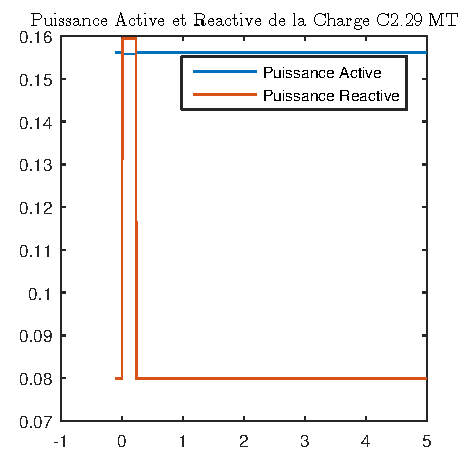
\includegraphics[width=0.475\textwidth]{Resultats/meus_resultados/Puissance_Active_et_Reactive_de_la_Charge_C2_29_MT}}
   \hfill
   \only<2>{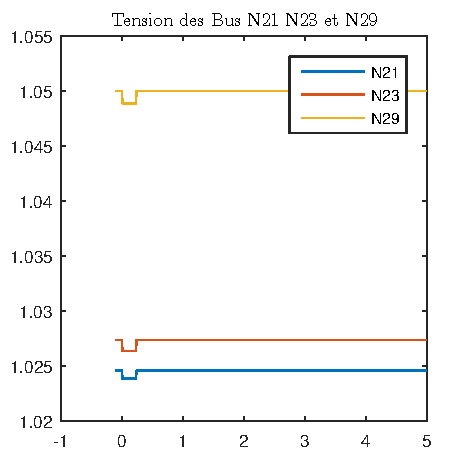
\includegraphics[width=0.475\textwidth]{Resultats/meus_resultados/Tension_des_Bus_N21_N23_et_N29}}\note<2>{Ca était fait pour chaque charge et chaque bus et matrice a était fait\\Le tableaux serait trop petit, c'est pas coherant}
\end{figure}
\end{frame}

\begin{frame}{Matrice de Gain}\centering
			\resizebox{0.5\textwidth}{!}{\begin{tabular}{cccccc}
		$\frac{V_{N01}}{Q_{C 2-19}}$& $\frac{V_{N02}}{Q_{C 2-19}}$& $\frac{V_{N19}}{Q_{C 2-19}}$& $\frac{V_{N20}}{Q_{C 2-19}}$&$ \cdots $&$\frac{V_{N32}}{Q_{C 2-19}}$\\
		&&&&&\\
		$ \vdots $&$ \vdots $&$ \vdots $&$ \vdots $&$ \ddots $&$ \vdots $\\
		&&&&&\\
		$\frac{V_{N01}}{Q_{C 2-27.1}}$& $\frac{V_{N02}}{Q_{C 2-27.1}}$& $\frac{V_{N19}}{Q_{C 2-27.1}}$& $\frac{V_{N20}}{Q_{C 2-27.1}}$&$ \cdots $&$\frac{V_{N32}}{Q_{C 2-27.1}}$\\
		&&&&&\\
		$\frac{V_{N01}}{Q_{C 2-27.2}}$& $\frac{V_{N02}}{Q_{C 2-27.2}}$& $\frac{V_{N19}}{Q_{C 2-27.2}}$& $\frac{V_{N20}}{Q_{C 2-27.2}}$&$ \cdots $&$\frac{V_{N32}}{Q_{C 2-27.2}}$\\
		&&&&&\\				
		$\frac{V_{N01}}{Q_{C 2-27.3}}$& $\frac{V_{N02}}{Q_{C 2-27.3}}$& $\frac{V_{N19}}{Q_{C 2-27.3}}$& $\frac{V_{N20}}{Q_{C 2-27.3}}$&$ \cdots$&$\frac{V_{N32}}{Q_{C 2-27.3}}$\\
		&&&&&\\
		$\frac{V_{N01}}{Q_{C 2-28}}$& $\frac{V_{N02}}{Q_{C 2-28}}$& $\frac{V_{N19}}{Q_{C 2-28}}$& $\frac{V_{N20}}{Q_{C 2-28}}$&$\cdots$&$\frac{V_{N32}}{Q_{C 2-28}}$\\
		&&&&&\\
		$ \vdots $&$ \vdots $&$ \vdots $&$ \vdots $&$ \ddots $&$ \vdots $\\
		&&&&&\\
		$\frac{V_{N01}}{Q_{C 2-32.1}}$& $\frac{V_{N02}}{Q_{C 2-32.1}}$& $\frac{V_{N19}}{Q_{C 2-32.1}}$& $\frac{V_{N20}}{Q_{C 2-32.1}}$&$\cdots$&$\frac{V_{N32}}{Q_{C 2-32.1}}$\\
		&&&&&\\
		$\frac{V_{N01}}{Q_{C 2-32.2}}$& $\frac{V_{N02}}{Q_{C 2-32.2}}$& $\frac{V_{N19}}{Q_{C 2-32.2}}$& $\frac{V_{N20}}{Q_{C 2-32.2}}$&$\cdots$&$\frac{V_{N32}}{Q_{C 2-32.2}}$\\
\end{tabular}}		
\end{frame}

\subsection{Simulation}
\begin{frame}{Simulation}\note{Pour faciliter la visualisation les prochains graphiques seront d'un seul générateur\\Tension en MegaVolts et temps en secondes}
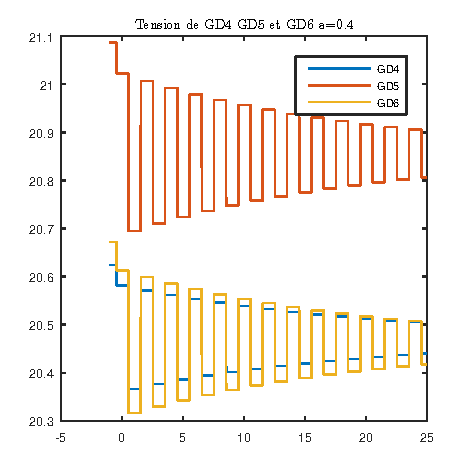
\includegraphics[width=0.3\textwidth]{Resultats/meus_resultados/Tension_de_GD4_GD5_et_GD6_a0_4.pdf}
\hfill
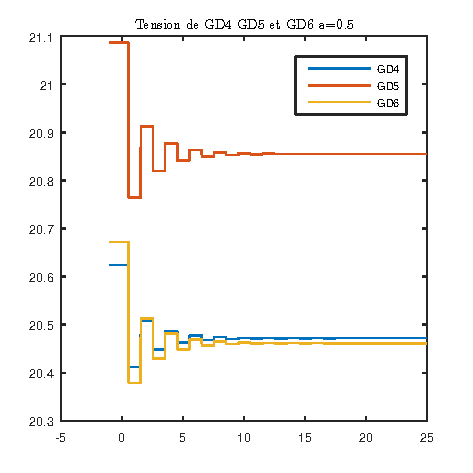
\includegraphics[width=0.3\textwidth]{Resultats/meus_resultados/Tension_de_GD4_GD5_et_GD6_a0_5.pdf}
\hfill
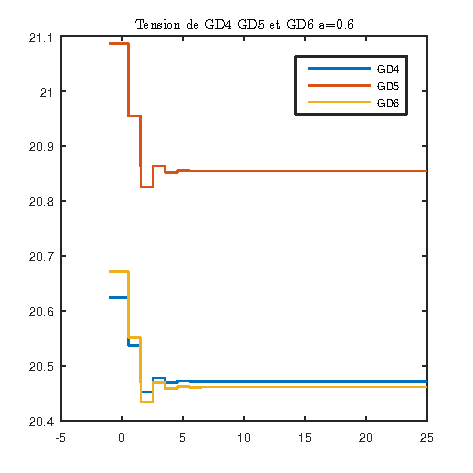
\includegraphics[width=0.3\textwidth]{Resultats/meus_resultados/Tension_de_GD4_GD5_et_GD6_a0_6.pdf}
\quad \\\quad\\ \centering \small  Sans Perturbation
\end{frame}

\begin{frame}{Simulation}
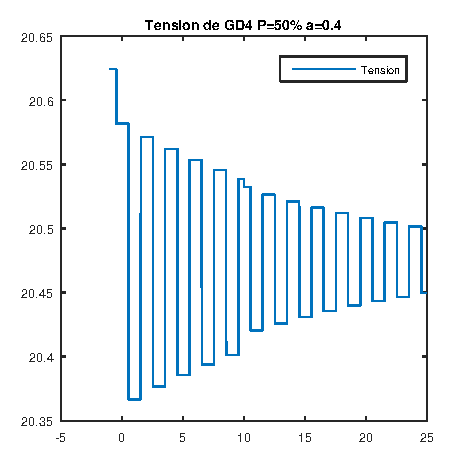
\includegraphics[width=0.3\textwidth]{Resultats/meus_resultados/Tension_de_GD4_P50_a0_4.pdf}
\hfill
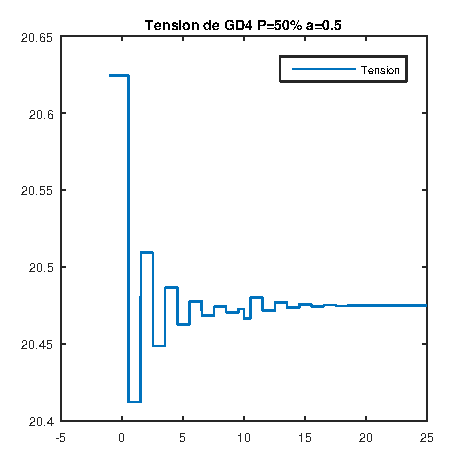
\includegraphics[width=0.3\textwidth]{Resultats/meus_resultados/Tension_de_GD4_P50_a0_5.pdf}
\hfill
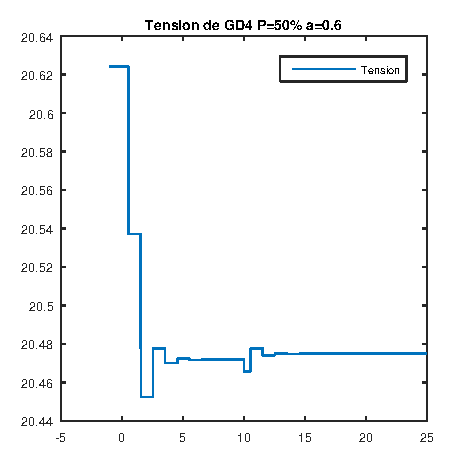
\includegraphics[width=0.3\textwidth]{Resultats/meus_resultados/Tension_de_GD4_P50_a0_6.pdf}
\quad \\\quad\\ \centering \small  Changement de Puissance Active en +50\%\\ Charge C2\_29\_MT
\end{frame}

\begin{frame}{Simulation}
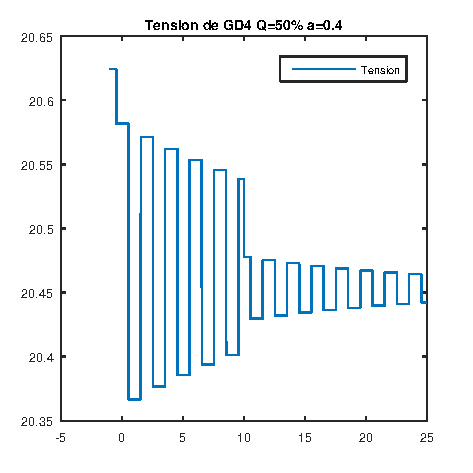
\includegraphics[width=0.3\textwidth]{Resultats/meus_resultados/Tension_de_GD4_Q50_a0_4.pdf}
\hfill
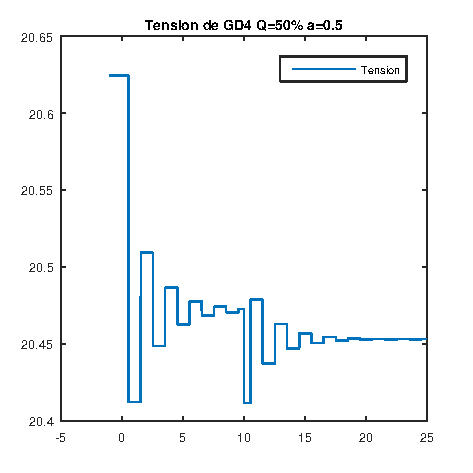
\includegraphics[width=0.3\textwidth]{Resultats/meus_resultados/Tension_de_GD4_Q50_a0_5.pdf}
\hfill
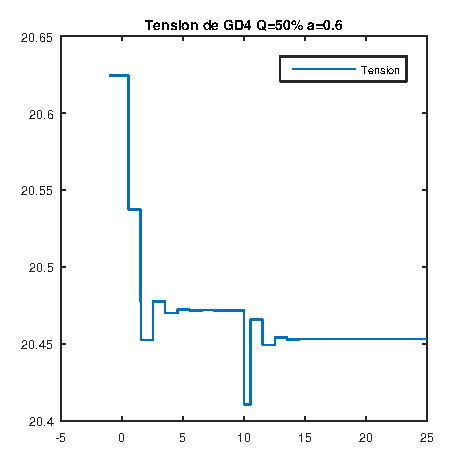
\includegraphics[width=0.3\textwidth]{Resultats/meus_resultados/Tension_de_GD4_Q50_a0_6.pdf}
\quad \\\quad\\ \centering \small  Changement de Puissance Réactive +50\%\\ Charge C2\_29\_MT
\end{frame}

\begin{frame}{Simulation}
	\centering
	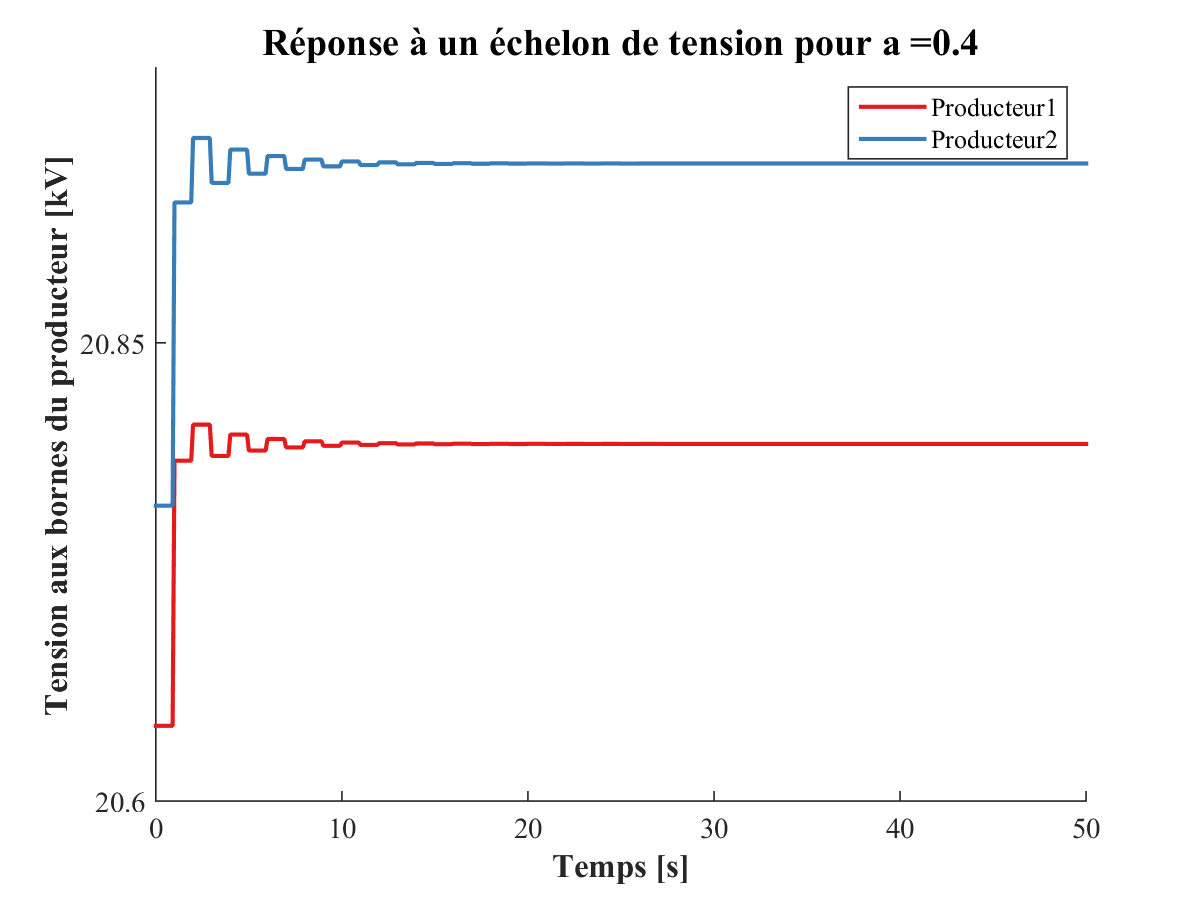
\includegraphics[width=0.3\linewidth]{Resultats/Cosson/Modele_Dyn_2_prod_a_40}\qquad
	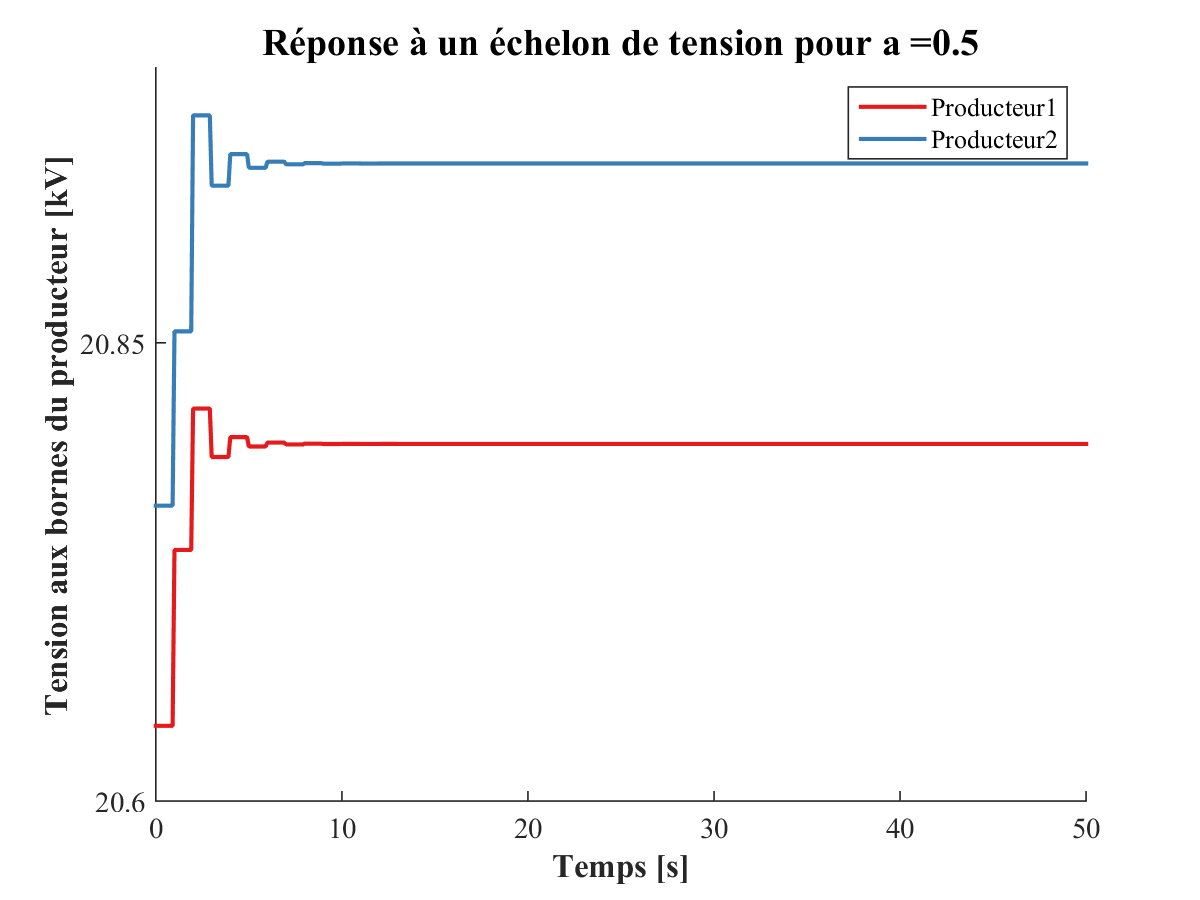
\includegraphics[width=0.3\linewidth]{Resultats/Cosson/Modele_Dyn_2_prod_a_50}
	\\\vspace{1em}
	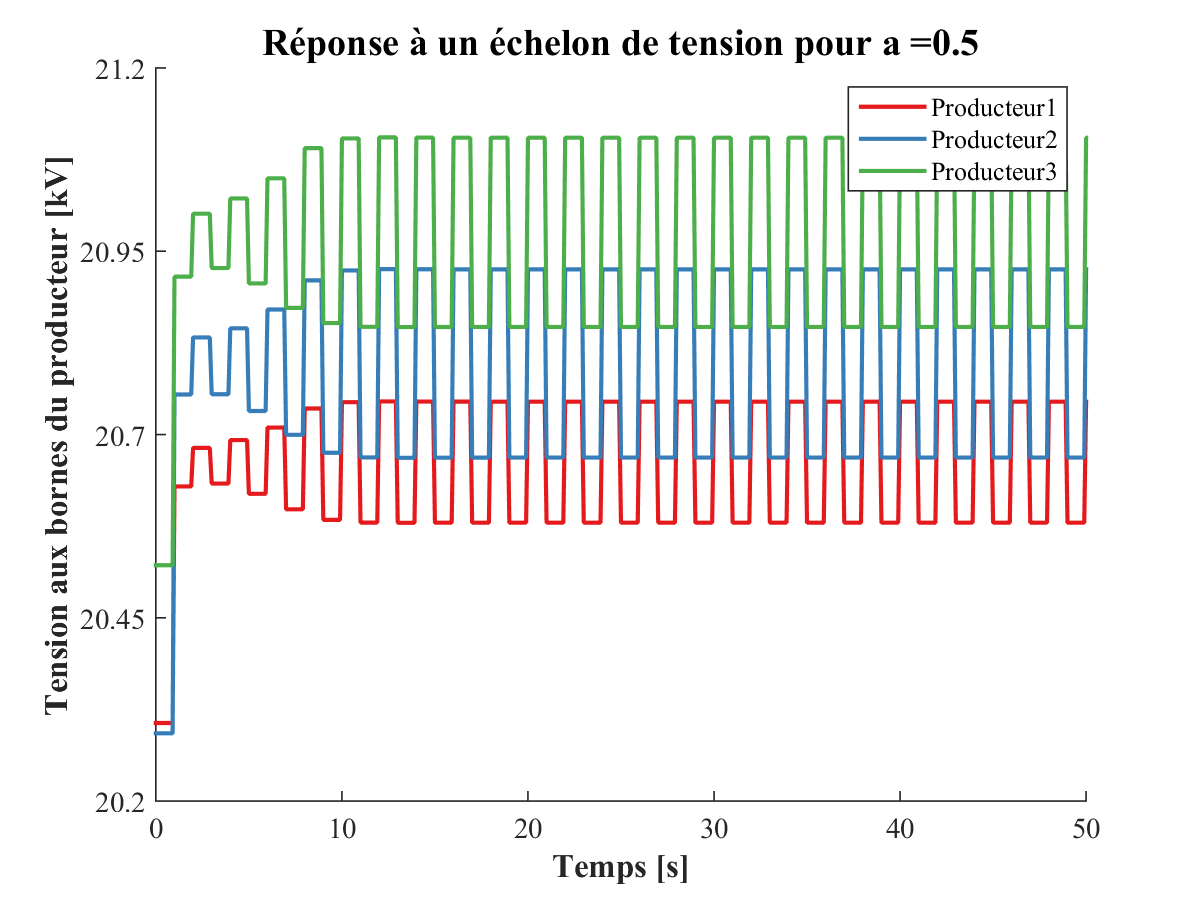
\includegraphics[width=0.3\linewidth]{Resultats/Cosson/Modele_Dyn_3_prod_a_50}\qquad
	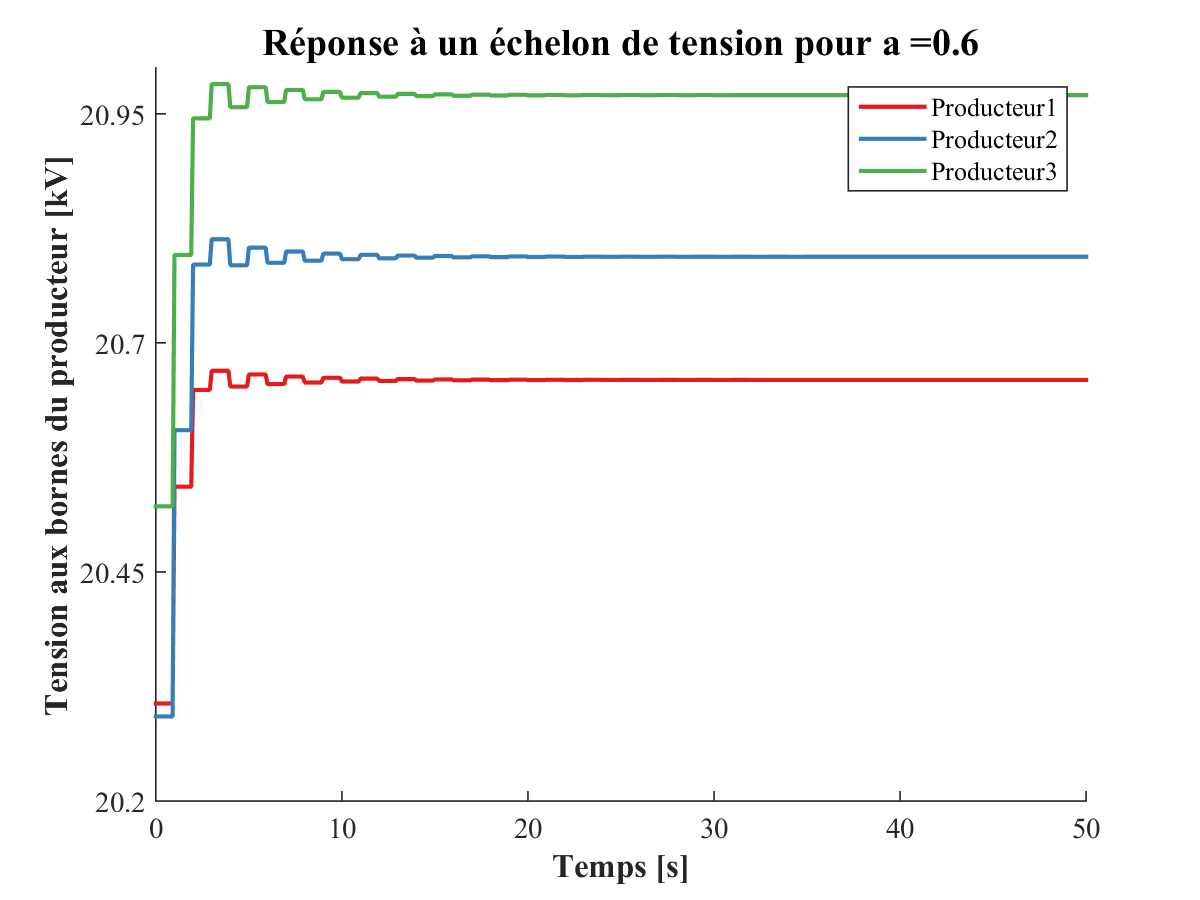
\includegraphics[width=0.3\linewidth]{Resultats/Cosson/Modele_Dyn_3_prod_a_60}
\end{frame}



